%================================================================
\documentclass[symmetry,article,submit,moreauthors,pdftex]{Definitions/mdpi} 

%=================================================================
% MDPI internal commands
\firstpage{1} 
\makeatletter 
\setcounter{page}{\@firstpage} 
\makeatother
\pubvolume{1}
\issuenum{1}
\articlenumber{0}
%\doinum{}
\pubyear{2021}
\copyrightyear{2020}
%\externaleditor{Academic Editor: Firstname Lastname} % For journal Automation, please change Academic Editor to "Communicated by"
\datereceived{} 
\dateaccepted{} 
\datepublished{} 
%\datecorrected{} % Corrected papers include a "Corrected: XXX" date in the original paper.
%\dateretracted{} % Corrected papers include a "Retracted: XXX" date in the original paper.
\hreflink{https://doi.org/} % If needed use \linebreak
%=================================================================
%% Please use the following mathematics environments: Theorem, Lemma, Corollary, Proposition, Characterization, Property, Problem, Example, ExamplesandDefinitions, Hypothesis, Remark, Definition, Notation, Assumption
%% For proofs, please use the proof environment (the amsthm package is loaded by the MDPI class).
\usepackage{listings}
\usepackage{subfigure}
%=================================================================
% Full title of the paper (Capitalized)
\Title{Optimal Fuzzy Controller Design for Autonomous Robot Path Tracking using Genetic Algorithms}

% MDPI internal command: Title for citation in the left column
\TitleCitation{Title}

% Author Orchid ID: enter ID or remove command
\newcommand{\orcidauthorA}{0000-0003-0430-8152} % Add \orcidA{} behind the author's name
\newcommand{\orcidauthorB}{0000-0002-2593-1114} % Add \orcidB{} behind the author's name
\newcommand{\orcidauthorC}{0000-0002-7385-5689} % Add \orcidB{} behind the author's name
\newcommand{\orcidauthorD}{0000-0002-1385-9741} % Add \orcidB{} behind the author's name

% Authors, for the paper (add full first names)
\Author{Alejandra Mancilla $^{1}$\orcidA{},
  Mario Garc\'{i}a-Valdez $^{1,}$*\orcidB{},
  Oscar Castillo$^{1}$\orcidC{} 
  and JJ Merelo-Guerv\'{o}s$^{2}$\orcidD{}}

% MDPI internal command: Authors, for metadata in PDF
\AuthorNames{Alejandra Mancilla, Mario Garc\'{i}a-Valdez, Oscar Castillo and JJ Merelo-Guerv\'{o}s}

% MDPI internal command: Authors, for citation in the left column
\AuthorCitation{Mancilla, A.; Garc\'{i}a-Valdez, M.; Castillo, O.; Merelo-Guerv\'{o}s, J.J.}
% If this is a Chicago style journal: Lastname, Firstname, Firstname Lastname, and Firstname Lastname.

% Affiliations / Addresses (Add [1] after \address if there is only one affiliation.)
\address{%
$^{1}$ \quad Tijuana Institute of Technology;\{alejanda.mancilla,mario,ocastillo\}@tectijuana.edu.mx\\
$^{2}$ \quad University of Granada; jmerelo@ugr.es}

% Contact information of the corresponding author
\corres{Correspondence: mario@tectijuana.edu.mx; Tel.:+52-664-123-7806 (M.G.V.)}

% Current address and/or shared authorship
%\simplesumm{} % Simple summary

\conference{INFUS-21} % An extended version of a conference paper

% Abstract (Do not insert blank lines, i.e. \\)

\abstract{ In this work we propose, through the use of a population-based
metaheuristic, an optimization method that solves the problem of autonomous path
tracking using a rear-wheel fuzzy logic controller. This approach enables the
design of controllers using rules that are linguistically familiar to human
users. Moreover, a new technique that uses three different paths to validate the
performance of each candidate configuration is presented. We extend on our
previous work by adding two more membership functions to the previous fuzzy
model, intending to have a finer-grained adjustment. Experiments show that,
compared to a published control law, % control law? - JJ
the proposed fuzzy controller has a better RMSE-measured performance but also
has limitations with respect to undesired yaw oscillation. Nevertheless, the
experiments also highlight problems with the common practice of evaluating the
performance of fuzzy controllers with a single problem case and performance
metric, resulting in controllers that tend to be overtrained.}

% Keywords
\keyword{Fuzzy Systems; Fuzzy Control; Bioinspired Algorithms.} 

\begin{document}

\section{Introduction}

Proposed by Lofti Zadeh \cite{goguen_zadeh_1973}, fuzzy logic introduces the
concepts of fuzzy sets and fuzzy logic operators \cite{zadeh1996fuzzy}.
Contrary to boolean logic, in which an element is a member of a set or is not,
now elements have a degree of membership to many sets. Fuzzy logic uses
so-called membership functions (MFs) to assign a numerical value to each set
member, indicating their degree of membership. MFs must be defined for each
linguistic variable; these variables can be used in a rule-based system to
express knowledge in a way similar to natural language, for instance, the rule
``if distance is near'' uses the linguistic variable distance, with a fuzzy MF
assigning a degree of membership to the set near to each element of the
distance domain; for instance, for 2mm and 50mm the function will assign the
following degrees of membership: near(2)=.92 and near(50)=.40. These rule based
systems can express complex relationships well suited for control applications.

That is why, since the earlier years of fuzzy logic theory, fuzzy inference
systems \cite{driankov_introduction_2013} have been applied to control problems
\cite{mamdani1974application,king1977application,passino1998fuzzy,driankov_introduction_2013},
in many research projects \cite{yang_improved_2003,driankov_fuzzy_2013} and
commercial systems.

An essential caveat of applying fuzzy control strategies to real-world problems
is that we require the use of optimization or adaptive techniques to tune some
aspects of the fuzzy inference system.  From the membership functions (MFs)
that define the linguistic variables to the rule definition of the rule-based
system, including the defuzzification method
\cite{xia2019command,isaka1988design}. 

Tuning is needed because the fuzzy controllers' performance is highly dependent
on the parameters of the fuzzy system used. Moreover, the option of making a
manual selection of these parameters is difficult because the search space is
of considerable size and requires the validation of establishing the
controller's performance by running time-consuming simulations.  Evolutionary
algorithms (EAs) and other metaheuristics are often employed in tuning FISs % Define this. Is it Fuzzy inference systems? - JJ
\cite{martinez-soto_bio-inspired_2012}. 

EAs are a kind of optimization metaheuristic used for solving complex
combinatorial problems \cite{back1993overview} with applications in many
engineering areas \cite{mateos_algoritmos_2004}.  One of the most common EAs
are Genetic Algorithms (GAs) \cite{holland1992genetic} which are
population-based search methods that are inspired in natural selection. In this
model, surviving individuals reproduce through genetic crossover and mutation
operators to generate offspring, and there is a replacement mechanism to select
the most adapted offspring \cite{muelas_algoritmos_2009}. GAs work on a set of
potential solutions called a population that is evolved for a certain number of
generations until a suitable or optimal solution is found. Even if this
combination of techniques is the basis of computational intelligence
\cite{wan1970applying,engelbrecht2007computational}, and there are many
contributions on the subject, there are still many application areas that have
specific requirements and challenges that have not been addressed or considered
by earlier works.

Many papers address the problem of path tracking control with fuzzy logic, the
earlier works used simple fuzzy rules to make adjustments to linear controllers
\cite{lee_practical_2003}, or integrated fuzzy logic to a complex adaptive
controller \cite{sanchez1997adaptive}. Meng \cite{bi_control_2020} proposes a
Fuzzy PID % Explain acronym too - JJ
algorithm to a two-degree-of-freedom arm robot. Antonin et al.
\cite{antonelli_fuzzy-logic-based_2007} propose a set of rules to emulate the
way humans drive, using as inputs of curve and distance to the system.  We have
also reviewed works where authors use controllers for the follow-up and
planning of routes. For example, using a simplified kinematic model of the
bicycle type using the control law for the navigation and follow-up of a route
\cite{laumond_robot_1998}, in work presented by Beleño et al.
\cite{beleno_planeacion_2014} they propose the planning and tracking of the
trajectories of a land vehicle based on the steering control in a natural
environment.  Guerrero-Castelanos et al.
\cite{guerrero-castellanos_trajectory_2014} addresses the path following
problem for the robot (3, 0) based on its kinematic model and proposes a
solution by designing a control strategy that mainly considers the maximum
permitted levels of the control signal. 

We have found in the literature various studies that optimize the parameters of
a fuzzy controller applied to mobile autonomous robots using different
bio-inspired metaheuristics
\cite{hernandez_optimization_2019,lagunes_methodology_2017}.  Wagner and Hagras
\cite{wagner2007genetic} propose a GA to evolve the architecture of a type-2
fuzzy controller in robot navigation for real environments; they optimize the
standard deviation of Gaussian type-2 MFs.  Again a GA is presented by Wu \&
Wan Tan \cite{wu2006genetic} for evolving the parameters of all the MFs of a
coupled-tank liquid-level control system.  Astudillo et al.
\cite{astudillo2013optimization} propose a new metaheuristic based on chemical
reactions to tune the parameters of a fuzzy controller for a uni-cycle robot.
There is also work focused on the metaheuristic optimization of fuzzy type-2
controllers, the main works are reviewed by Castillo
\cite{castillo_review_2012}, and the main reason for using this type of
controller is to model the uncertainty of the sensor data or the fuzzy model
itself.


We have observed that most of these studies optimize the parameters of MFs
directly. For instance, if we have a triangular function for a fuzzy set $A$,
defined by a lower limit $a$, and upper limit of $b$ and a value $m$ where $a <
m <b$ as 

\begin{equation}\label{eq:triangular}
\mu_{trian}(x) = 
\begin{cases}
    0, & x \le a \\
    \frac{x-a}{m-a}, & a < x \le m \\ 
    \frac{b-x}{b-m}, & m < x \le b \\ 
    0, & x \ge b
\end{cases},
\end{equation}

each value is optimized independently, sometimes validating only the
restriction $a < m <b$. In this work, we propose a method that adds further
restrictions, including symmetric definition and limiting the range of values
of each parameter. In our previous work, we compared symmetrical and
asymmetrical definitions and found that symmetrical restrictions give better
results for rear-wheel-based controllers. 

The main contribution of this work is to propose, through the use of a
population-based metaheuristic, an optimization method to solve the problem of
autonomous path tracking using a rear-wheel controller in the framework of
fuzzy logic. This approach enables the design of controllers using rules that
are linguistically familiar to human users.

Therefore, following the preliminary work in
\cite{mancilla2022tracking,Mancilla2021}, in this paper we propose the
addition of a more granular definition of fuzzy variables by including two more
membership functions. Also, we propose a new parametrization technique that
enables the definition of symmetric MFs, by using an aperture factor instead of
the previous method that used a delta from a fixed point.  These additions
greatly improve the controller's evolutionary design by significantly
decreasing the tracking error (RMSE) compared to our previous work. We also
propose a new evaluation method for establishing the fitness of candidate
solutions by using three different trajectories in each simulation.
Experimental results show that this method reduces the risk of generating an
over-trained controller with low error for a specific track but cannot function
in other paths. To demonstrate the application of the method, we report an
experimental case study using a bicycle-like mobile robot with nonholonomic
constraints. 

In this work, we choose the problem of trajectory tracking since it has the
particularity of being naturally symmetric since the error is measured by
moving away either to the left or right of the desired path. Furthermore, in
the literature, we have not found applications of fuzzy systems to follow the
trajectory of a route so that this research could solve similar problems.

We structure this document as follows: in Section~\ref{MatAndMethods}, we
present the proposed method, configurations, and we describe the experimental
setup. In Section~\ref{Results} we present the results achieved, and finally,
in Section~\ref{Discussion} we discuss the results and highlight future
research directions.

%The introduction should briefly place the study in a broad context and
%highlight why it is important. It should define the purpose of the work and its
%significance. The current state of the research field should be reviewed
%carefully and key publications cited. Please highlight controversial and
%diverging hypotheses when necessary. Finally, briefly mention the main aim of
%the work and highlight the principal conclusions. As far as possible, please
%keep the introduction comprehensible to scientists outside your particular
%field of research. Citing a journal paper \cite{castillo_new_2015}. Now citing a book
%reference \cite{paden_survey_2016,fortin_deap_2012} or other reference types.
 
%%%%%%%%%%%%%%%%%%%%%%%%%%%%%%%%%%%%%%%%%%
\section{Materials and Methods}\label{MatAndMethods}

\subsection{Rear-Wheel Feedback and Kinematic Model}

In this work, we use a simplified model of a bicycle-type kinematic robot
consisting of two wheels connected by a rigid link of size $l$ with
nonholonomic restrictions \cite{pamucar_vehicle_2018,de1998feedback}.  The
front-wheel can steer in the axis normal to the plane of motion, the steering
angle is $\delta$ (see Figure \ref{fig:kinematics}), The position of the
midpoint of the rear-wheel is given by the coordinates $x_r$ and $y_r$. The
heading $\theta$ is the angle of the link between the two wheels and the $x$
axis.  We follow the model describe in \cite{paden_survey_2016}, with the
differential constraint:

\begin{equation}
    \begin{matrix}
        \dot{x}_{r}  = v_r \cos (\theta),\\ 
        \dot{y}_{r}  = v_r \sin (\theta),\\
        \dot{\theta} = \frac{v_r}{l} \tan (\delta).
    \end{matrix}
\end{equation}

The controller selects the steering angle $\delta$ with a value between the
limits of the vehicle $\delta \in [\delta_{min},\delta_{max}]$ and a desired
velocity $v_r$ again limited by $v\in [v_{min},v{max}]$. The heading rate
$\omega$ is related to the steering angle by 

\begin{equation}
       \delta = \arctan \left(\frac{l\omega}{v_r}\right),
\end{equation}

and we can simplify the heading dynamics to 

\begin{equation}
    \dot{\theta} = \omega,\quad \omega \in \left[\frac{v_r}{l} \tan(\delta_{min}),\frac{v_r}{l} \tan(\delta_{max} ) \right].
\end{equation}.

\begin{figure}[H] 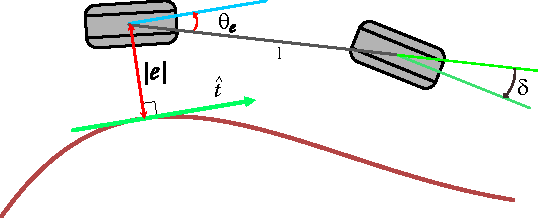
\includegraphics[width=10.5 cm]{img/path} \caption{ Feedback
        and actuator variables for the rear-wheel-based control. The magnitude
        of $e$ illustrated in red, is the error measured from the rear wheel to
        the nearest point on the path. When e > 0, the wheel is at the right of
        the path, and when e < 0 is at the left. $\theta_e$ is the
        difference between the tangent at the nearest point in the path and the
        the heading $\theta$. The output of the controller is the heading rate
        $\omega$, from which we calculate the steering angle $\delta$ of the front wheel.
}\label{fig:kinematics}    \end{figure} 

Now we explain the path tracking method described by Paden et al.
\cite{paden_survey_2016}.  This controller takes the feedback from the
rear-wheel position as Figure \ref{fig:kinematics} illustrates.  The path
(shown in red in the figure) is a continuous function with properties
described in \cite{samson1992path}, and the feedback is a function of the
nearest point on the reference path given by 

\begin{equation}
s(t) = \operatorname*{arg\,min}_{\gamma} \|(x_r(t),y_r(t)) - (x_{ref}(\gamma),y_{ref}(\gamma)) \|.
\end{equation}

and the tracking error vector is 

\begin{equation}
d(t) = (x_r(t),y_r(t))-(x_{ref}(s(t)),y_{ref}(s(t)))
\end{equation}

The heading error is based on a unit vector $\hat{t}$ (shown in green on Figure
\ref{fig:kinematics}) tangent to the path at $s(t)$ given by 

\begin{equation}
\hat{t} = \frac{ \left(\left.\frac{\partial x_{ref}}{\partial s} \right|_{s(t)},\left.\frac{\partial y_{ref}}{\partial s} \right|_{s(t)}\right)} 
              {\left\| \left(\frac{\partial x_{ref}(s(t))}{\partial s},\frac{\partial y_{ref}(s(t))}{\partial s}\right) \right\|},
\end{equation}

The error $e$ is the cross product of the two vectors

\begin{equation}
e = d_x \hat{t}_y - d_y \hat{t}_x
\end{equation}

The heading error uses the angle $\theta_e$ between the robot's heading vector
and $\dot(t)$

\begin{equation}
\theta_e(t) = \theta - arctan_2 \left( \frac{\partial x_{ref}(s(t))}{\partial s} , \frac{\partial y_{ref}(s(t))}{\partial s} \right)
\end{equation}



%The control law for  

%\begin{equation}
%\omega = \frac{v_r \mathcal{K}(s) \cos(\theta_e)}{1 - \mathcal{K}(s)e} - g_1(e, \theta_e,t)\theta_e - k_2v_r \frac{\sin(\theta_e)}{\theta_e}e,
%\end{equation}
%%

%Based on this model we nowfollowing a trajectory specified using cubic splines is
%described.
\subsection{Fuzzy Controllers}%
    \label{sub:FuzzyControllers}

To design a fuzzy controller from the model we just described, we must consider
the magnitude of the scalar value $e$, the distance from the rear wheel to the
route's closest point. This error is positive if it is on the right and
negative on the left of the route. Another input variable is the angle
$\theta_e$ defined between the heading vector and the tangent vector of the
route. This angle can also be negative or positive depending on the vehicle's
position concerning the route; the controller output is the heading rate
$\omega$, which allows us to calculate the steering angle $\delta$. The target
velocity of the robot will be constant, so we will not control the
velocity $v$ using the fuzzy controller we will use the following simple
proportional controller instead

\begin{equation}
    a = K_p(v_{ref}-v_r).
\end{equation}

In this work, we will compare two fuzzy models, one with three MFs, which was
proposed in our previous work \cite{Mancilla2021}, and a new model using five
MFs. We describe both fuzzy systems next.

\subsubsection{Fuzzy Model with Three Membership Functions}

We now model the same input and output variables mentioned above as fuzzy
variables using three membership functions. Each variable has the same fuzzy
values: high negative ({\tt hi\_neg}), low ({ \tt  low } ), and high positive
({ \tt hi\_pos}). Depending on the case, the sign indicates whether it is to
the right or left of the path. We use trapezoidal functions for the ``high''
fuzzy term (positive and negative) and a triangular function for the ``low''
value.

We consider a total membership in extreme values (depending on each variable's
domain). Because of this, we ignore the trapezoidal parameters' values outside
the value domain. In total, we could modify up to 33 parameters for all
membership functions. We propose keeping the extreme parameters outside the
domain and the central point of the triangular function fixed. The center of
the triangular functions will always be at 0 since it is the minimum error
possible.  We kept the fuzzy rules symmetrical, representing how a human driver
would adjust the steering wheel when driving. The rules are presented in Table~\ref{tab:3mf}.
We have nine rules, to establish a relation between all the
possible inputs and output values.

\begin{specialtable}[H]
    %\small
    \caption{Proposed fuzzy rules for the basic controller with three membership functions.}\label{tab:3mf}
    \centering
    \begin{tabular}{lllllll}
    Rule 1: & If $\theta_e$ is & { \tt hi\_neg} & and $e$ is & {\tt low}     & then $\omega$  is & {\tt hi\_pos}     \\
    Rule 2: & If $\theta_e$ is  & { \tt hi\_pos} & and $e$ is & {\tt low}     & then $\omega$ is & {\tt hi\_neg }    \\
    Rule 3: & If $\theta_e$ is & { \tt  low }     & and $e$ is & {\tt low}     & then $\omega$ is &{\tt low}         \\
    Rule 4: & If $\theta_e$ is & { \tt hi\_neg} & and $e$ is & {\tt hi\_neg} & then $\omega$ is &{\tt hi\_pos}     \\
    Rule 5: & If $\theta_e$ is & { \tt hi\_pos} & and $e$ is & {\tt hi\_pos} & then $\omega$ is &{\tt hi\_neg }    \\
    Rule 6: & If $\theta_e$ is & { \tt hi\_pos} & and $e$ is & {\tt hi\_neg} & then $\omega$ is &{\tt low   }      \\
    Rule 7: & If $\theta_e$ is & { \tt hi\_neg} & and $e$ is & {\tt hi\_pos} & then $\omega$ is & {\tt low   }      \\
    Rule 8: & If $\theta_e$ is & { \tt low }    & and $e$ is & {\tt hi\_pos} & then $\omega$ is & {\tt hi\_neg }    \\
    Rule 9: & If $\theta_e$ is & { \tt low}     & and $e$ is & {\tt hi\_neg} & then $\omega$ is & {\tt hi\_pos }
    \end{tabular}
 \end{specialtable}


\subsubsection{Fuzzy Model with Five Membership Functions}

We now add two more membership functions to the previous fuzzy model, intending
to have a finer grain of adjustment. Adding more functions also adds more
complexity to the rules, and now we have even more parameters to tune.  Instead
of having just two values for each type of error { \tt hi } and {\tt low} we
add a middle value, represented by the { \tt medium } membership function. The
knowledge in the fuzzy rule base is now more complex than before, with 25
rules. In this case, defining the rules was not done by simply specifying a
driver's knowledge. We needed to adjust the rules by running several
simulations. The rules are presented in Table~\ref{tab:5mfRules}.

\begin{specialtable}[H]
    \caption{Proposed fuzzy rules for the basic controller with three membership functions.}\label{tab:5mfRules}
    \centering
    \begin{tabular}{lllllll}
    Rule 1:  & If $\theta_e$ is & { \tt hi\_neg}  & and $e$ is  & { \tt hi\_neg}  &	then $\omega$ is & { \tt hi\_pos}  \\
    Rule 2:  & If $\theta_e$ is & { \tt hi\_neg}  & and $e$ is	& { \tt med\_neg} &	then $\omega$ is & { \tt hi\_pos}  \\
    Rule 3:  & If $\theta_e$ is & { \tt hi\_neg}  & and $e$ is  & { \tt low}      &	then $\omega$ is & { \tt hi\_pos}  \\
    Rule 4:  & If $\theta_e$ is & { \tt hi\_neg}  & and $e$ is	& { \tt med\_pos} &	then $\omega$ is & { \tt med\_pos} \\
    Rule 5:  & If $\theta_e$ is & { \tt hi\_neg}  & and $e$ is	& { \tt hi\_pos}  &	then $\omega$ is & { \tt low}      \\
    Rule 6:  & If $\theta_e$ is & { \tt med\_neg} & and $e$ is	& { \tt hi\_neg}  &	then $\omega$ is & { \tt med\_pos} \\
    Rule 7:  & If $\theta_e$ is & { \tt med\_neg} & and $e$ is	& { \tt med\_neg} &	then $\omega$ is & { \tt med\_pos} \\
    Rule 8:  & If $\theta_e$ is & { \tt med\_neg} & and $e$ is	& { \tt low}      &	then $\omega$ is & { \tt med\_pos} \\
    Rule 9:  & If $\theta_e$ is & { \tt med\_neg} & and $e$ is	& { \tt med\_pos} &	then $\omega$ is & { \tt med\_pos} \\
    Rule 10: & If $\theta_e$ is	& { \tt med\_neg} & and $e$ is	& { \tt hi\_pos}  &	then $\omega$ is & { \tt low}      \\
    Rule 11: & If $\theta_e$ is	& { \tt low}      &	and $e$ is	& { \tt hi\_neg}  &	then $\omega$ is & { \tt hi\_pos}  \\
    Rule 12: & If $\theta_e$ is	& { \tt low}      &	and $e$ is	& { \tt med\_neg} &	then $\omega$ is & { \tt low}      \\
    Rule 13: & If $\theta_e$ is	& { \tt low}      &	and $e$ is	& { \tt low}      &	then $\omega$ is & { \tt low}      \\
    Rule 14: & If $\theta_e$ is	& { \tt low}      &	and $e$ is	& { \tt med\_pos} &	then $\omega$ is & { \tt low}      \\
    Rule 15: & If $\theta_e$ is	& { \tt low}      &	and $e$ is	& { \tt hi\_pos}  &	then $\omega$ is & { \tt hi\_neg}  \\
    Rule 16: & If $\theta_e$ is	& { \tt med\_pos} &	and $e$ is	& { \tt hi\_neg}  &	then $\omega$ is & { \tt low}      \\
    Rule 17: & If $\theta_e$ is	& { \tt med\_pos} &	and $e$ is	& { \tt med\_neg} &	then $\omega$ is & { \tt med\_neg} \\
    Rule 18: & If $\theta_e$ is	& { \tt med\_pos} &	and $e$ is	& { \tt low}      &	then $\omega$ is & { \tt med\_neg} \\
    Rule 19: & If $\theta_e$ is	& { \tt med\_pos} &	and $e$ is	& { \tt med\_pos} &	then $\omega$ is & { \tt med\_neg} \\
    Rule 20: & If $\theta_e$ is	& { \tt med\_pos} &	and $e$ is  & { \tt hi\_pos}  &	then $\omega$ is & { \tt med\_neg} \\
    Rule 21: & If $\theta_e$ is	& { \tt hi\_pos}  &	and $e$ is	& { \tt hi\_neg}  &	then $\omega$ is & { \tt low}      \\
    Rule 22: & If $\theta_e$ is	& { \tt hi\_pos}  &	and $e$ is	& { \tt med\_neg} &	then $\omega$ is & { \tt med\_neg} \\
    Rule 23: & If $\theta_e$ is	& { \tt hi\_pos}  &	and $e$ is	& { \tt low}      &	then $\omega$ is & { \tt hi\_neg}  \\
    Rule 24: & If $\theta_e$ is	& { \tt hi\_pos}  &	and $e$ is	& { \tt med\_pos} &	then $\omega$ is & { \tt hi\_neg}  \\
    Rule 25: & If $\theta_e$ is	& { \tt hi\_pos}  &	and $e$ is	& { \tt hi\_pos}  &	then $\omega$ is & { \tt hi\_neg}    
       
    \end{tabular}
 \end{specialtable}

\subsection{Tuning of Parameters Using a Genetic Algorithm}%
    \label{sec:GA}

As we mentioned earlier, the proposed fuzzy controllers we proposed in the
previous Section~\ref{sub:FuzzyControllers} need to be tuned to give
acceptable results on a simulation. In this section, we describe our proposed
method for MFs parameter optimization. First, we need to establish which
parameters we are going to keep fixed and which parameters we are going to
tune. The following two sections explain the parameter selection and the
overall technique. 

\subsubsection{ Parameter Tuning for Three MFs configuration}

In this configuration, we modified the input and output variables' parameters
symmetrically, varying the minimum extremes of the trapezoidal functions 

\begin{equation}\label{eq:trapezoidal}
\mu_{trap}(x) = \max{ \left( \min{ \left( \frac{x-a}{b-a},1,\frac{d-x}{d-c} \right)}, 0 \right)}  
\end{equation}

where the trapezoidal begins to descend/ascend and the point where it reaches zero.

We varied these parameters symmetrically $(a, b, d, e, g, h)$; in the case of
the triangular function (\ref{eq:triangular}), the aperture we symmetrically
optimized $(c, f, i)$ the parameters as shown in Table~\ref{tab:paramsTriang}.
To keep the symmetry, we just repeat the same parameter value on both sides of
a triangular function or on the values of the trapezoidal. Some values are used
only to make the function broader or narrower at the bottom. In this case, we
parameterize the controller with just nine variables, and these are the
parameters that the GA will optimize. That we will explain in
Section~\ref{sec:GA}.

\begin{specialtable}[htbp]
    \small
    \caption{Nine parameter configuration for three MFs fuzzy controller.}\label{tab:paramsTriang}
    \begin{tabular}{cccc}
    \toprule
    \textbf{Variable} & \textbf{Linguistic Value} & \textbf{MF}& \textbf{Parameters}  \\
    \midrule
    $\theta_e$ & high negative  & $\mu_{trap}$  & $[-100, -100, -a, -a+b]$     \\ 
    $\theta_e$ & low            & $\mu_{tria}$  & $[-c, 0, c]$     \\ 
    $\theta_e$ & high positive  & $\mu_{trap}$  & $[a+b, a, 100, 100]$     \\ 

    \midrule
    $error$ & high negative  & $\mu_{trap}$  & $[-100, -100, -d, -d+e]$     \\ 
    $error$ & low            & $\mu_{tria}$  & $[-f, 0, f]$     \\ 
    $error$ & high positive  & $\mu_{trap}$  & $[d+e, d, 100, 100]$     \\ 

    \midrule
    $omega$ & high negative  & $\mu_{trap}$  & $[-8, -8, -g, -g+h]$     \\ 
    $omega$ & low            & $\mu_{tria}$  & $[-i, 0, i]$     \\ 
    $omega$ & high positive  & $\mu_{trap}$  & $[g+h, g, 8, 8]$     \\ 
    \bottomrule
\end{tabular}
\end{specialtable}.


\subsubsection{ Parameter Tuning for Five MFs configuration}

In a similar fashion as before, we need to define which parameters will be
tuned for the five MFs controller. Again we keep the MFs symmetrical around
zero. In this case, we just needed ten variables to parameterize the
controller. To achieve this, we kept the parameters of $\omega$ fixed. The
parameters are illustrated in Figure~\ref{tab:5mf}.

\begin{specialtable}[htbp]
    \small
    \caption{Ten parameter configuration for five MFs fuzzy controller.}\label{tab:5mf}
    \begin{tabular}{cccc}
    \toprule
     \textbf{Variable} & \textbf{Linguistic Value} & \textbf{MF}& \textbf{Parameters}  \\
    \midrule
    $\theta_e$ & high negative  & $\mu_{trap}$  & $[-50, -5, -b, -b+c]$     \\ 
    $\theta_e$ & medium negative& $\mu_{tria}$  & $[-d-e, -d, -d+e]$     \\ 
    $\theta_e$ & low            & $\mu_{tria}$  & $[-a, 0, a]$     \\ 
    $\theta_e$ & medium positive& $\mu_{tria}$  & $[-d-e, d, d+e]$     \\ 
    $\theta_e$ & high positive  & $\mu_{trap}$  & $[b-c, b, 5, 50]$ \\

    \midrule
    $error$ & high negative  & $\mu_{trap}$  & $[-50, -5, -g, -g+h]$     \\ 
    $error$ & medium negative& $\mu_{tria}$  & $[-i-j, -i, -i+j]$     \\ 
    $error$ & low            & $\mu_{tria}$  & $[-f, 0, f]$     \\ 
    $error$ & medium positive& $\mu_{tria}$  & $[-i-j, i, i+j]$     \\ 
    $error$ & high positive  & $\mu_{trap}$  & $[g-h, g, 5, 50]$ \\

    \midrule
    $\omega$ & high negative  & $\mu_{trap}$  & $[-50, -5, -1, -0.5]$     \\ 
    $\omega$ & medium negative& $\mu_{tria}$  & $[-1, -0.5, 0]$     \\ 
    $\omega$ & low            & $\mu_{tria}$  & $[-0.5, 0, 0.5]$     \\ 
    $\omega$ & medium positive& $\mu_{tria}$  & $[0, 0.5,1]$     \\ 
    $\omega$ & high positive  & $\mu_{trap}$  & $[0.5, 1 ,5, 50]$     \\ 
    \bottomrule
\end{tabular}
\end{specialtable}

\subsubsection{ Parameter Tuning for Three MFs configuration}

Another essential aspect to consider when tuning the above parameters is the
range of values that each parameter can have. Normally, we keep all the
parameters in the same range when using a population-based metaheuristic. In
our previous work, we compared two ranges of values for the first controller,
with ranges $[0,1]$ and $[0,2]$. Our experiments showed better results with the
narrower range, so we selected the same configuration for the three MFs
controllers for this work. In this work, we propose a simple technique to
change the tuning ranges for the MFs while keeping the adjustable parameters in
the same range of values $[0,1]$. We define different ranges for the input
variables and normalize the values before they are passed to the membership
functions.  These values are shown in Table~\ref{tab:factor}.

\begin{specialtable}[H] 
\small
\caption{Ranges defined for each parameter for the 5MF controller.}\label{tab:factor}
\begin{tabular}{clcl}
\toprule
\textbf{Parameter}	& \textbf{Range}& \textbf{Parameter} & \textbf{Range}\\
\midrule
a & [0,1]			& f & [0, 1]\\
b & [0.5,2]			& g & [0.5, 2]\\
c & [0,2]			& h & [0, 2]\\
d & [0.5,1.5]		& i & [0.5,1.5]\\
e & [0,1]			& j & [0, 1]\\
\bottomrule
\end{tabular}
\end{specialtable}

\subsubsection{Genetic Algorithm Optimization}\label{sec:GAO}

As a population-based metaheuristic, the GA needs to evaluate the fitness of
each candidate solution (also called individuals) in its population. This
process is illustrated in Figure~\ref{fig:ga}. Each candidate solution is
represented by a chromosome, here implemented as a list of objects of type {
\tt float }. To evaluate each solution, we need to generate an instance of the
fuzzy controller. The membership functions are defined using the parameters
included in the chromosome. Once created, the fuzzy controller is passed as a
parameter, together with the tracks the mobile robot will follow. The output of
the simulations is the RMSE of the accumulated errors $e$  obtained during the
simulations. We consider this measure as the fitness of the candidate solution.
The GA will not select the candidate solutions with the worst fitness for
reproduction.

\begin{figure}[H]
\centering
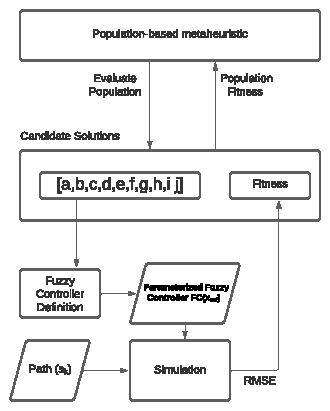
\includegraphics[width=9 cm]{img/ga}
\caption{
For each individual in the population, a controller is created with the
parameters, this controller is then tested by running one or more simulations.
The RMSE of the tracking is considered as the fitness for that particular
candidate solution. This process is repeated for each member of the
population.
}\label{fig:ga}
\end{figure} 


In our previous work \cite{Mancilla2021} we evolved the controllers with a
single path; we noticed that this could lead to over-training. Similar to what
happens in supervised learning algorithms, the controller found by the GA could
be specialized only to the track used for its evolution. We found that the
controller with only three MFs could follow new unseen tracks, but this was not
the case for the five MFs controller. It is well known that in rule-based
learning, adding more rules can harm the capacity to generalize to unseen
problems \cite{tan2016introduction}. Noticing this, we added a list of three
tracks to evaluate the fitness for the experiments, which is the average RMSE
of the three simulations. We ran experiments with one and three tracks. We
defined each track using cubic splines over a list of coordinates; this is a
common approach in the literature \cite{zhang2013cubic}. The tracks and the
parameters to define them are shown in Table~\ref{tab:routes}. The first track
was used on previous work and was taken from the library of
\cite{sakai_pythonrobotics_2018}, this track starts with a very narrow curve to
the left that is difficult for controllers to follow, but it remains
differentiable throughout the path, we call this track ``M''. The other tracks
are called ``A'' and ``S'' and have smoother curves, with long straight
segments and different curvatures. All tracks have seven anchor points for the
cubic spline.

\begin{specialtable}[H] 
\small
\caption{Tracks used for fitness evaluation, they are defined by cubic splines with the parameters shown below each plot.\label{tab:routes}}
\begin{tabular}{lll}
\toprule
\multicolumn{1}{c}{\textbf{Track M}}		& \multicolumn{1}{c}{\textbf{Track A}}& \multicolumn{1}{c}{\textbf{Track S}}\\
\midrule
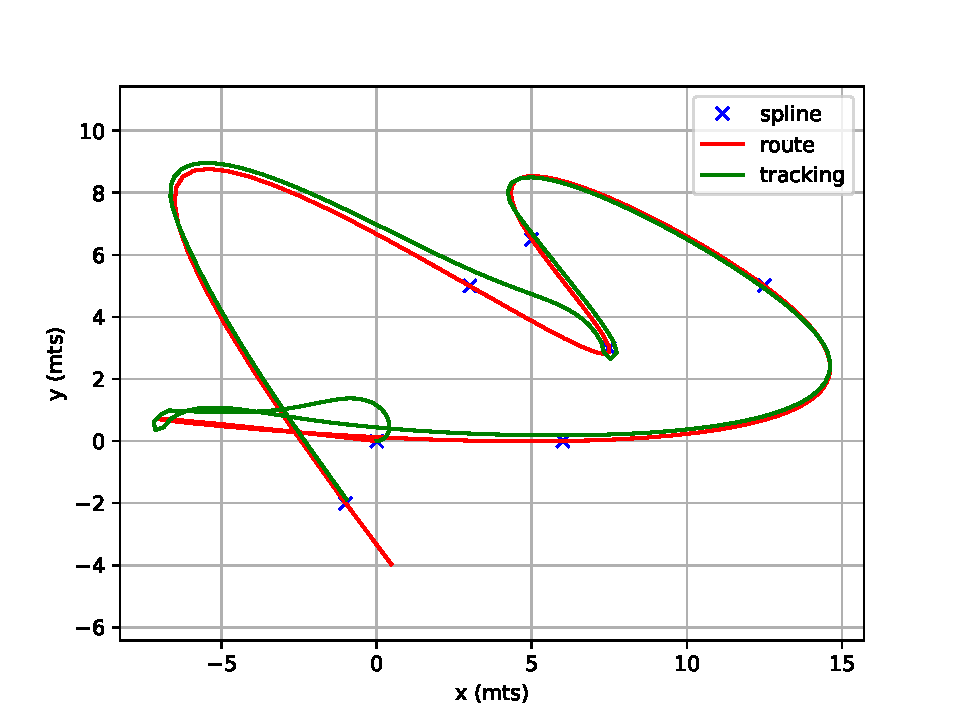
\includegraphics[scale=0.23]{img/M.pdf}& 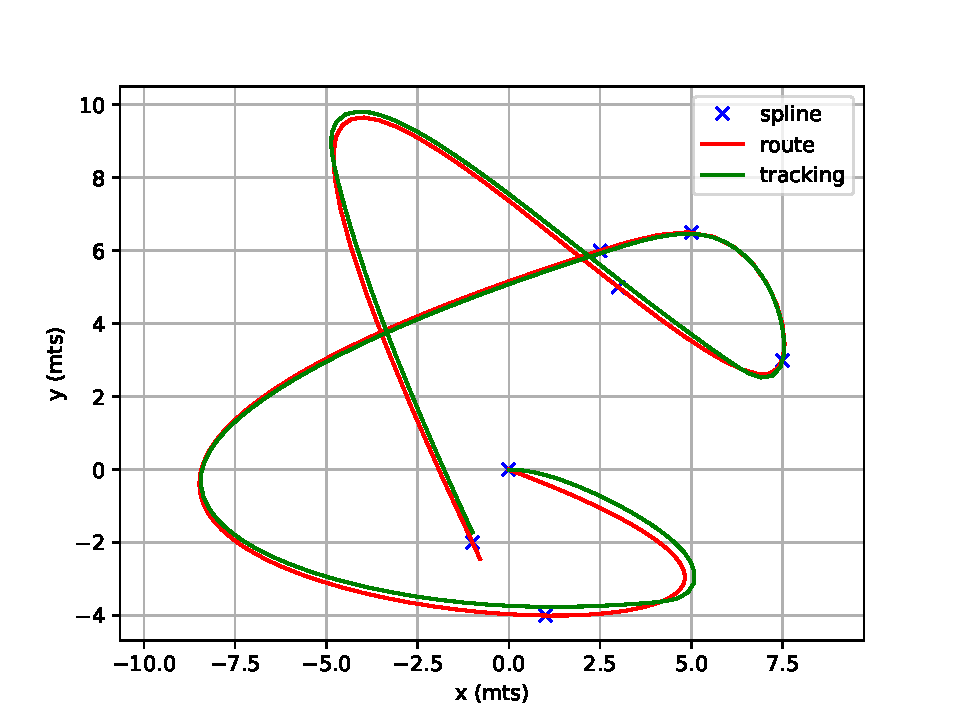
\includegraphics[scale=0.23]{img/A.pdf} & 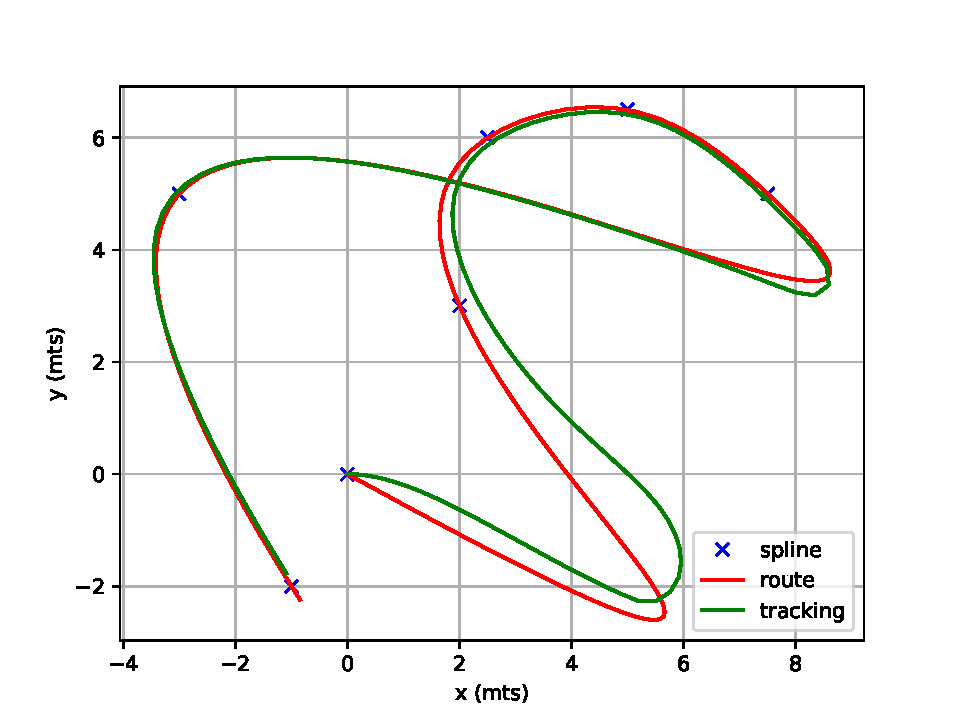
\includegraphics[scale=0.23]{img/S.pdf}\\
  $ax=[0,6,12,5,7.5,3,-1]$	&$ax = [0, 1, 2.5, 5, 7.5, 3, -1] $& $ ax = [0, 2, 2.5, 5, 7.5, -3, -1]$\\
  $ay = [0, 0,  5, 6.5, 3, 5, -2]  $	&$ay = [0, -4, 6, 6.5, 3, 5, -2] $& $ ay = [0, 3, 6, 6.5, 5, 5, -2] $\\
\bottomrule
\end{tabular}
\end{specialtable}

\subsubsection{Experimental Setup} % (fold)
\label{sub:setup}

We implemented the algorithm in Python using the DEAP \cite{fortin_deap_2012}
library for the GA implementation. We used the scikit-fuzzy
\footnote{https://github.com/scikit-fuzzy/scikit-fuzzy} library to code the
fuzzy inference  systems. Finally, we modified a fork of the PythonRobotics
repository \cite{sakai_pythonrobotics_2018}, adding the odeint library from the
SciPy package \footnote{https://github.com/scipy/scipy} to integrate the system
of ordinary equations.

All experiments ran with the same parameters for the GA. The only obvious
difference was the size of the chromosomes because this is the same as the
number of parameters we need to optimize. As we mentioned earlier, we proposed
two controllers, one with three membership functions; we are going to call this
controller 3MF, and the other controller 5MF because it has five membership
functions. For details on these controllers, see
Section~\ref{sub:FuzzyControllers}.  After several preliminary experiments, we
settled for a configuration with a population size of 50 with 20 generations.
We used single-point crossover with $0.3$ probability.  We opted for tournament
selection with a tournament size of three. For mutation, and because we are
using continuous values, we selected a Gaussian mutation with $\mu=0.0$ and
$\sigma=0.2$. Finally, the probability for each gene to be mutated was $0.2$.
Each individual's fitness was the RMSE mentioned earlier, but to economize the
computational resources, while the simulations were running, we interrupted
those simulations where the robot was clearly out of the track or did not
finish near the final point of the track. In these cases, we assigned a very
low fitness (we want to minimize the error) of 5000 to the first case and 2000
to the second.  

As the basis for comparison, we compare or results against the controller in
\cite{paden_survey_2016}, with the following control law defined as 

\begin{equation}\label{eq:controller}
\omega = \frac{v_r \mathcal{K}(s) \cos(\theta_e)}{1 - \mathcal{K}(s)e} -
  (k_{\theta}|v_r|)\theta_e - \left( k_ev_r \frac{\sin(\theta_e)}{\theta_e}\right) e,
\end{equation}

the parameters of the simulations and the canonical controller we are comparing
against are summarized in Table~\ref{tab:sim_params}.

\begin{specialtable}[H] 
\small
\caption{Simulation and controller parameters.}\label{tab:sim_params}
\begin{tabular}{ll}
\toprule
\textbf{Parameter}	& \textbf{Value}\\
\midrule
Wheel-base & $l=2.5$		\\
Steering limit & $|\delta|\le \frac{\pi}{4}$	\\
Initial configuration & $x_r(0),y_r(0),\theta(0)= (0,0,0)$\\
Velocity controller configuration & $K_p=1, v(0)=0, a(0)=0$\\
Target velocity & $v_r=\frac{10}{3}$\\
Maximum time & 50 \\ 
Control law parameters&$k_e=0.3, k_{\theta}=1.0$\\ 
\bottomrule
\end{tabular}
\end{specialtable}

We ran the experiments on a Desktop PC with AMD Ryzen 9 3900x 12-core processor
with 24 threads and 48 GB RAM with Ubuntu Linux 21.04, and Python 3.7.5 code.
Code and data can be found in the following GitHub repository
\url{https://github.com/mariosky/fuzzy-control}.


% subsubsection (?4:_:\lGA)(?4:_:\l)(?4:_:\limplementation) (end)


%%%%%%%%%%%%%%%%%%%%%%%%%%%%%%%%%%%%%%%%%
\section{Results}\label{Results}

This section shows the results of running the GA optimization of parameters for
the two controllers described in the previous sections. We have the 3MF and 5MF
controllers by running the GA optimization 30 times, using the average of the
three tracks to establish the fitness.  Moreover, we also ran a GA for both
controllers using only the most challenging track (Track M) for the evaluation.
The descriptive statistics of these results are shown in
Table~\ref{tab:statistics}.  As expected, and because the optimization is
non-deterministic, there are a few outliers at both extremes of the
performance. However, the deviation is higher when using only one track for the
GAs evaluation. Nevertheless, the 5MF controller has the lower RMSE in both
experiments.  The problem we found and mentioned earlier is that the 5MF
controller trained with a single track can not follow the path of the other
tracks; this is not the case with the 3MF controller.  For this reason, we will
only consider the controller optimized with three tracks for further
comparison. In the last column, we have the average execution time in seconds,
for as expected, evaluating with three tracks is more time-consuming. However,
we can also observe that it takes more time to evolve the 5MF controller. 

\begin{specialtable}[H] 
\small
\caption{Descriptive statistics for 30 executions of the GA with an evaluation
    of one and three tracks.}\label{tab:statistics}
\begin{tabular}{llllll}
\toprule
\textbf{Evaluation} & \textbf{Controller} & \textbf{Average }	& \textbf{Standard } &\textbf{Median}	& \textbf{Average Exec. }\\
                    &                     & \textbf{RMSE}	& \textbf{ Deviation} &\textbf{}	& \textbf{Time (s)}\\
\midrule
Three tracks & MF3 & 0.4321 & 0.071 & 0.4136 & 1283s \\
Three tracks & MF5 & \textbf{0.0156} & 0.031 & 0.0091 & 2664s \\
\midrule
Single track & MF3 & 0.6831 & 0.1096 & 0.6866 & 533s \\
Single track & MF5 & \textbf{0.0330} & 0.1030 & 0.0055 & 640s \\
\bottomrule
\end{tabular}
\end{specialtable}

We selected the best controllers found in the 30 experiments and compared them
against a controller using the control law in Equation~\ref{eq:controller}.
This results are presented in Table~\ref{tab:rmse}. Again the controller 5FM
has the lower RMSE on all individual tracks. The 3MF controller has a similar
RMSE when we compare it against the control law.

\begin{specialtable}[H] 
\small
\caption{RMSE of the best controllers in all three tracks.}\label{tab:rmse}
\begin{tabular}{llll}
\toprule
\textbf{Track}	& \textbf{Control } &\textbf{3MF}	& \textbf{5MF}\\
	& \textbf{law} & & \\
\midrule
Route M & 2.003 & 0.820 & \textbf{0.003} \\
Route A & 0.014 & 0.016 & \textbf{0.005} \\
Route S & 0.521 & 0.162 & \textbf{0.008} \\
\bottomrule
\end{tabular}
\end{specialtable}



When we observe the optimized MFs for both controllers, 3MF in
Figure~\ref{fig:3mf} and 5MF in Figure~\ref{fig:5mf}, we can see that they are
similar on the \texttt{low} and \texttt{high} MFS, for both the $\theta_r$ and
$e$, moreover, in each of them both variables are very similar. With only omega
having very different parameters.  We can also see that the values of $\omega$
remain fixed on 5MF, because we kept those parameters fixed.

\end{paracol}
\begin{figure}[H]
    \widefigure
     \centering
    \subfigure[Optimized membership functions for the 3MF fuzzy controller.]{\label{fig:3mf}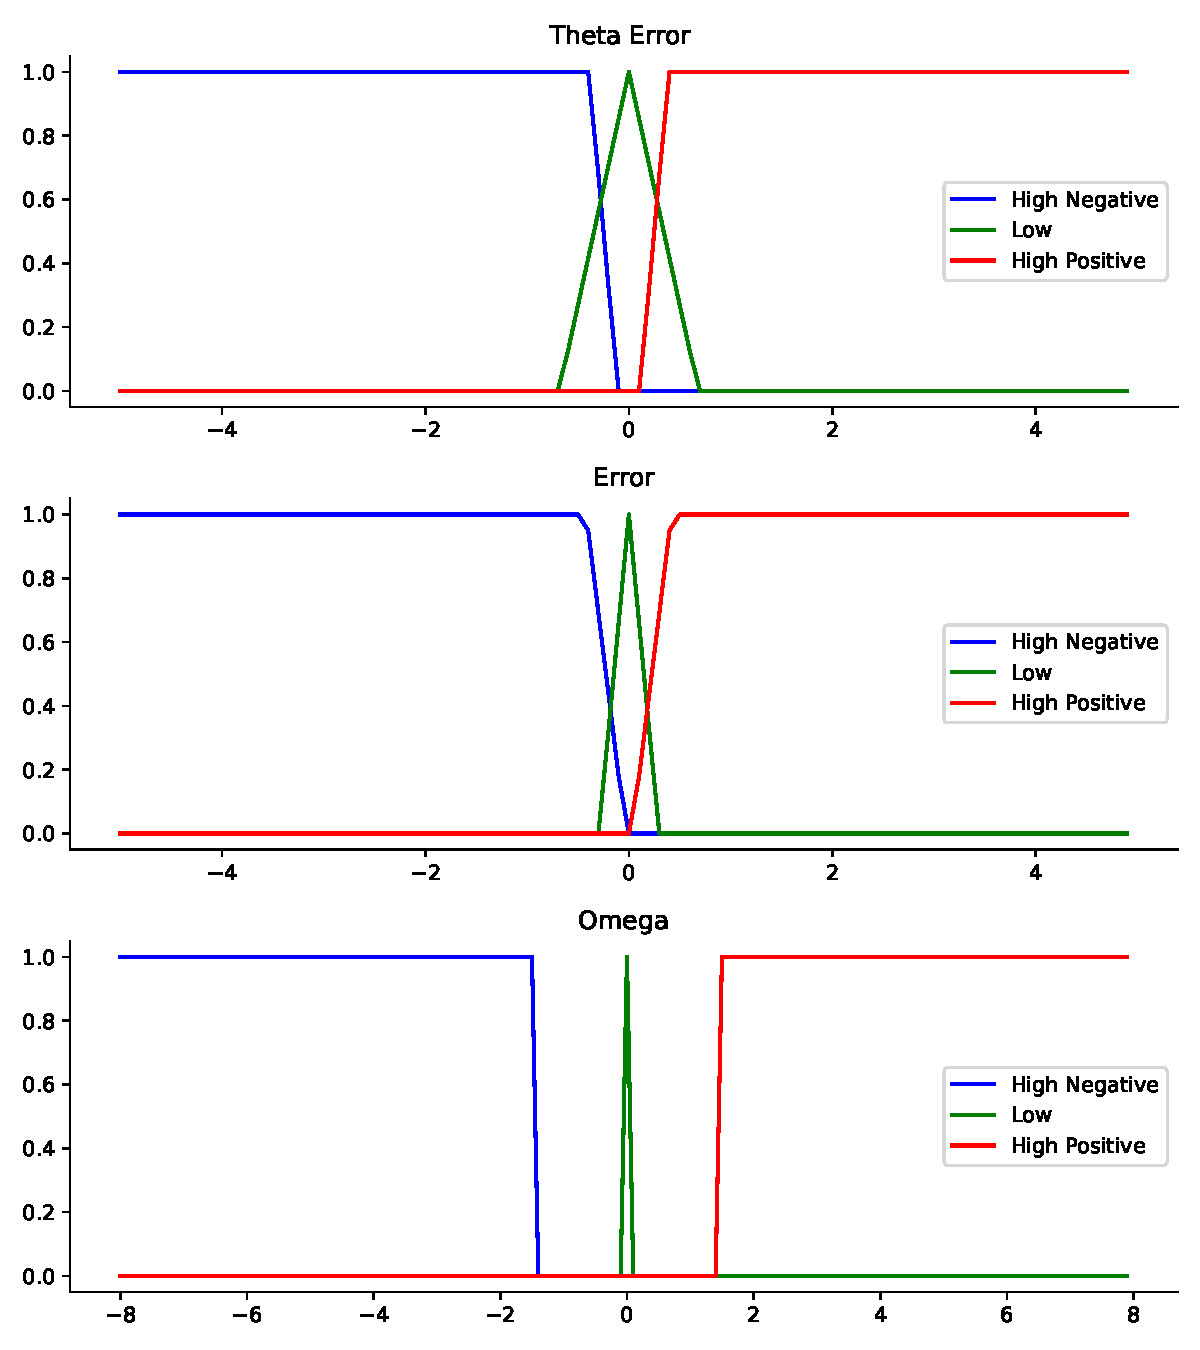
\includegraphics[width=90mm]{img/3r3fmR.pdf}}
    \subfigure[Optimized membership functions for the 5MF fuzzy controller.]{\label{fig:5mf}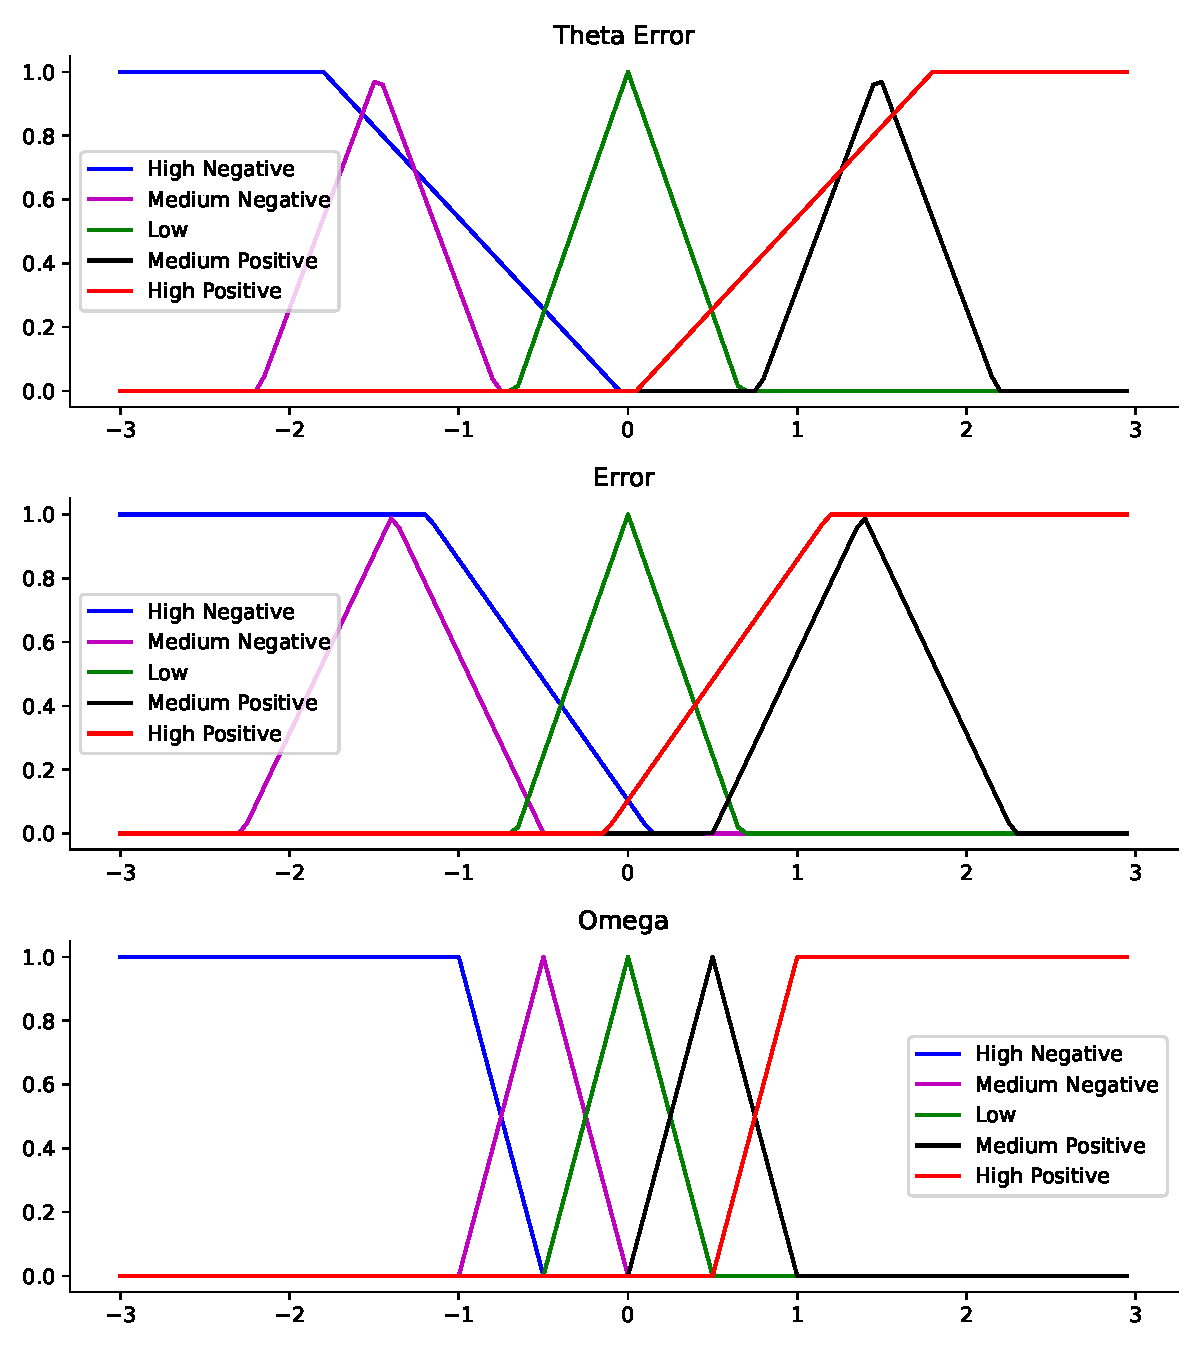
\includegraphics[width=90mm]{img/3r5fmR.pdf}}
     \caption{GA optimized membership functions for both controllers.}
        \label{fig:MFs}
\end{figure}
\begin{paracol}{2}
\linenumbers
\switchcolumn


We now show a plot of the tracks and the robot's movement following the track.
First, we have the track ``M'' (see Figure~\ref{fig:3RutasM}), in which all
controllers have problems at the beginning with a curve that is very sharp to
the left and then a sharp U-turn to go back to the start.  We can see that the
3MF controller follows the path with less zig-zag than controller 5MF, which
keeps the tracking closer to the path but with noticeable zig-zagging.

\end{paracol}
\begin{figure}[H]
    \widefigure
     \centering
    \subfigure[Control law]{\label{fig:compM}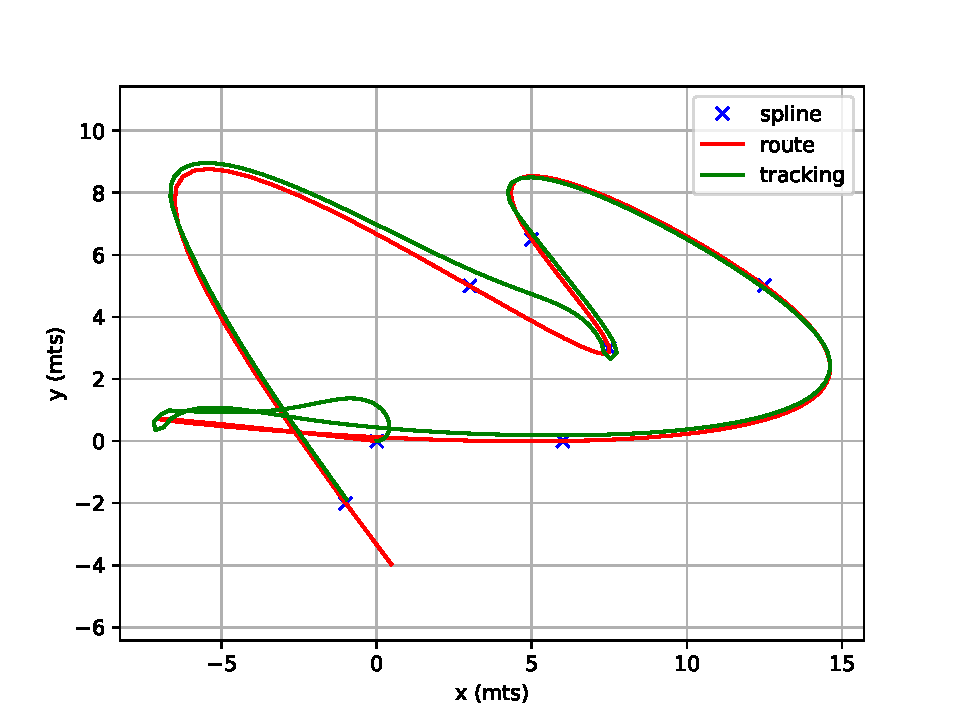
\includegraphics[width=60mm]{img/M.pdf}}
    \subfigure[3MF]{\label{fig:comp3MF}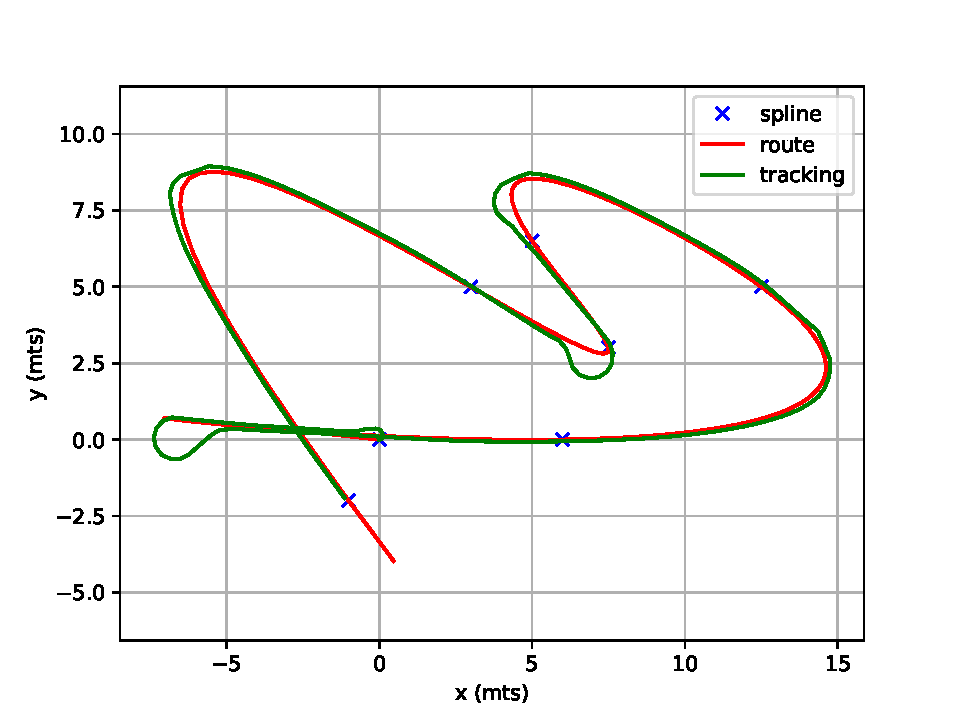
\includegraphics[width=60mm]{img/3r3fmM.pdf}}
    \subfigure[5FM]{\label{fig:comp5FM}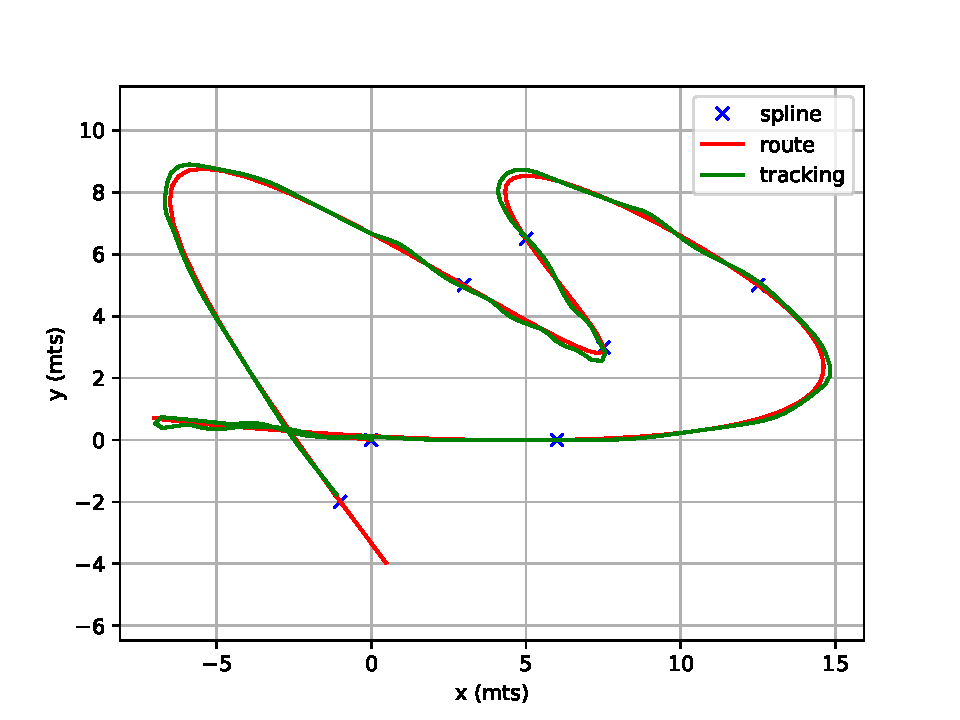
\includegraphics[width=60mm]{img/3r5fmM.pdf}}
     \caption{Plot for the best simulations on Track M}
        \label{fig:3RutasM}
\end{figure}
\begin{paracol}{2}
\linenumbers
\switchcolumn

The plots in Figure~\ref{fig:3RutasA} show the ``A'' track. This time all
controllers closely follow the path. Again controller 5MF has a noticeable
zig-zagging but manages to have the lower RMSE of the three.

\end{paracol}
\begin{figure}[H]
    \widefigure
     \centering
    \subfigure[Control law]{\label{fig:compA}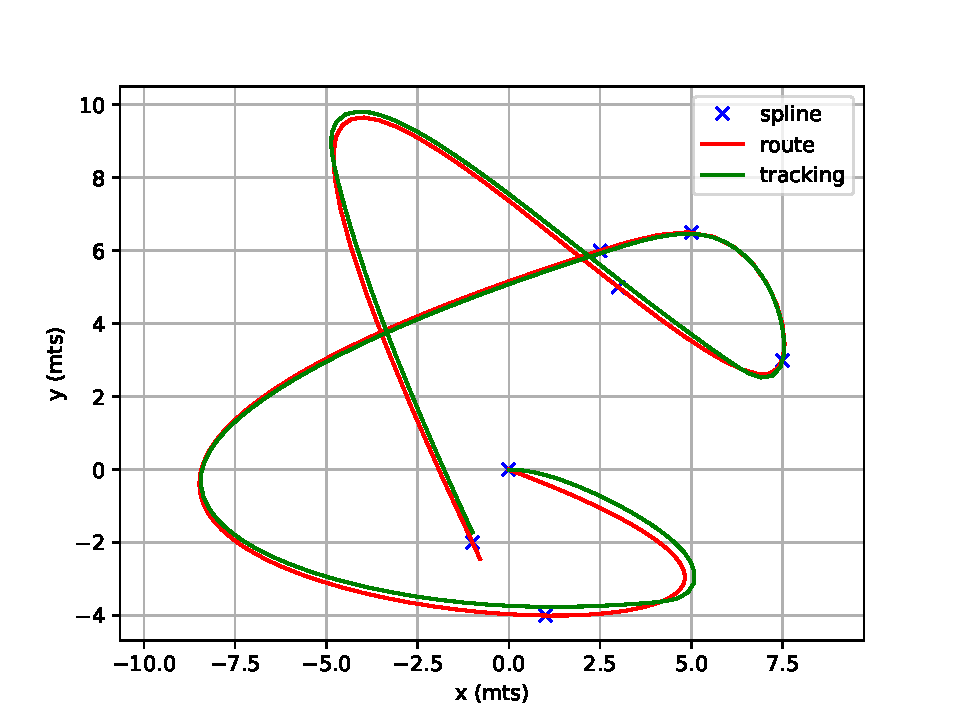
\includegraphics[width=60mm]{img/A.pdf}}
    \subfigure[3MF]{\label{fig:compA3MF}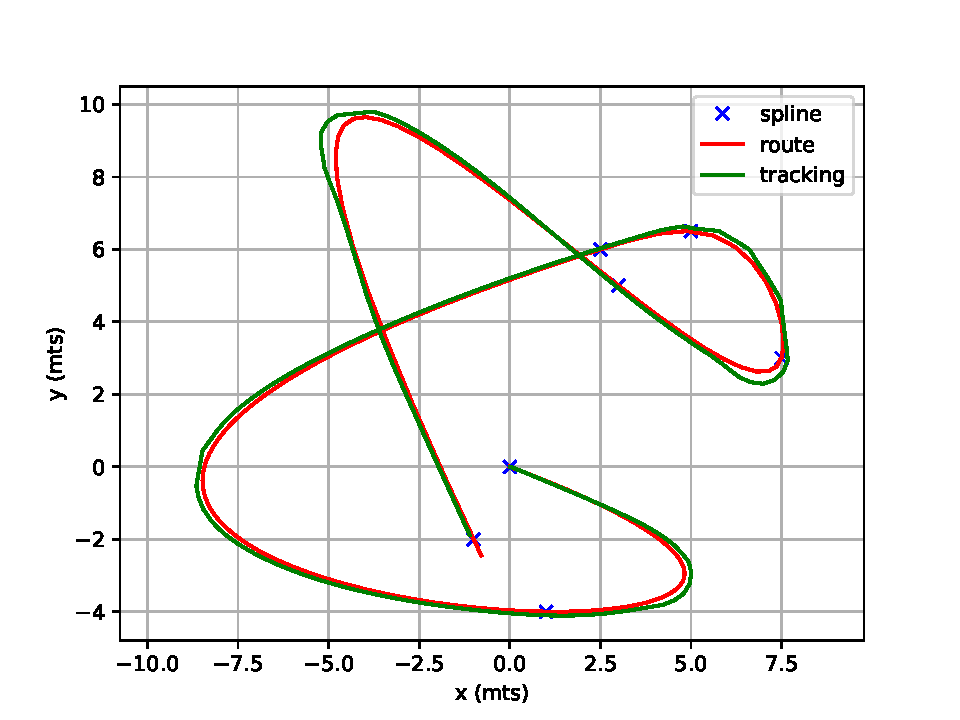
\includegraphics[width=60mm]{img/3r3fmA.pdf}}
    \subfigure[5FM]{\label{fig:compA5FM}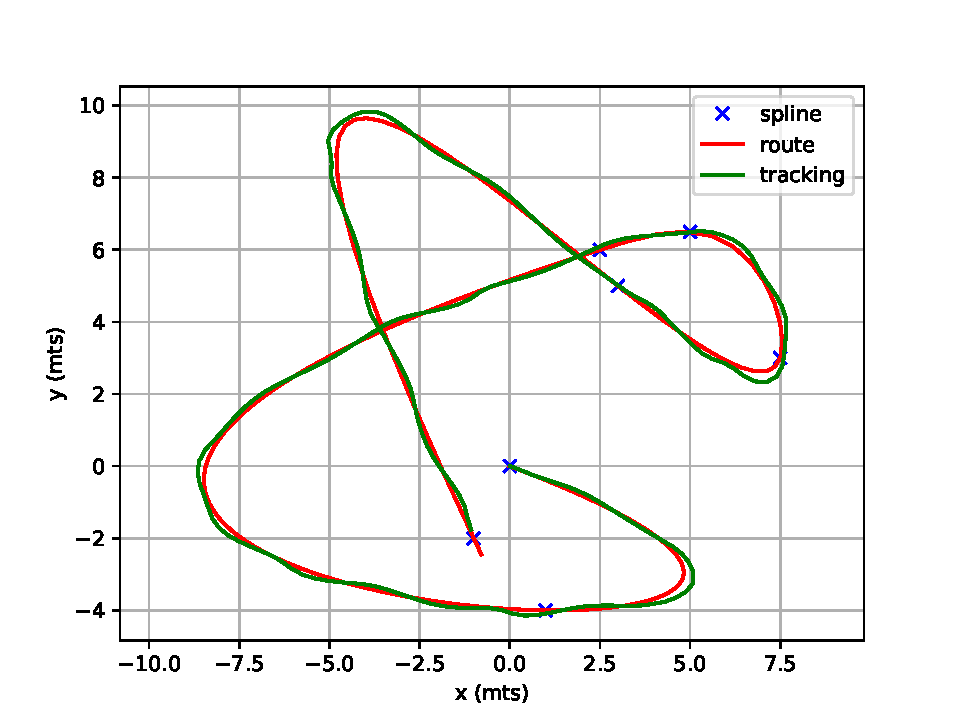
\includegraphics[width=60mm]{img/3r5fmA.pdf}}
     \caption{Plot for the best simulations on Track A}
        \label{fig:3RutasA}
\end{figure}
\begin{paracol}{2}
\linenumbers
\switchcolumn


The results of Figure~\ref{fig:3RutasS} highlight the overall behavior of the
three controllers. The control law takes more time to reach the path when it
deviates from the reference because it has smoother steering, but once it is
over the track, $e$ does not increase.  That is by design because one of the
conditions is that a small initial tracking error will remain small. On the
other hand controller 3MF, does not deviate much from the reference, has a
smoother control than the 5MF, but it has a higher RMSE.

\end{paracol}
\begin{figure}[H]
    \widefigure
     \centering
    \subfigure[Control law]{\label{fig:compS}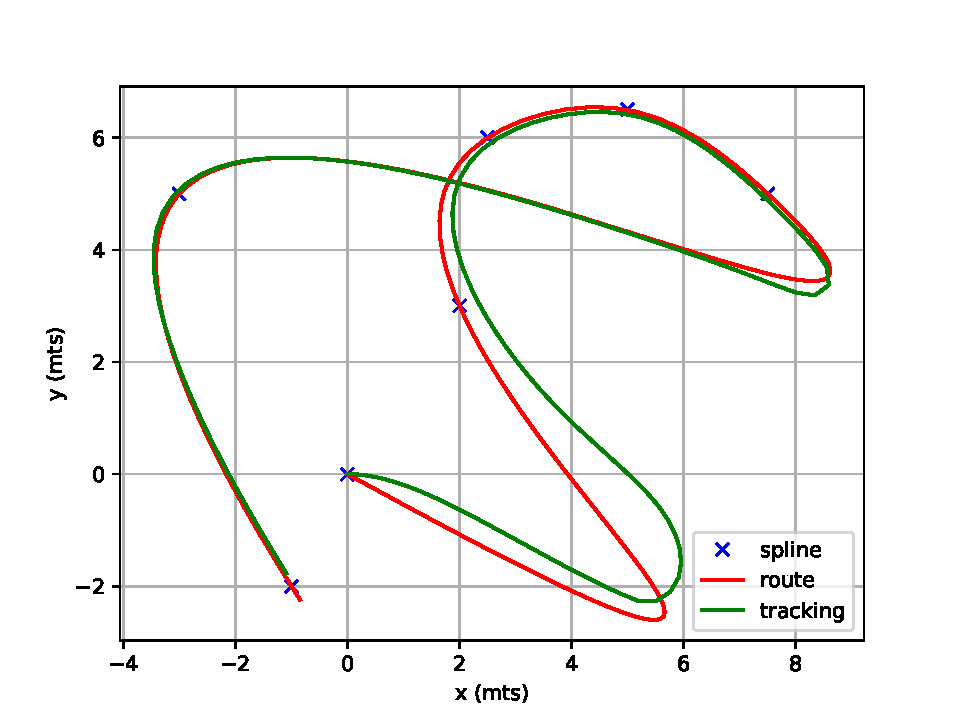
\includegraphics[width=60mm]{img/S.pdf}}
    \subfigure[3MF]{\label{fig:compS3MF}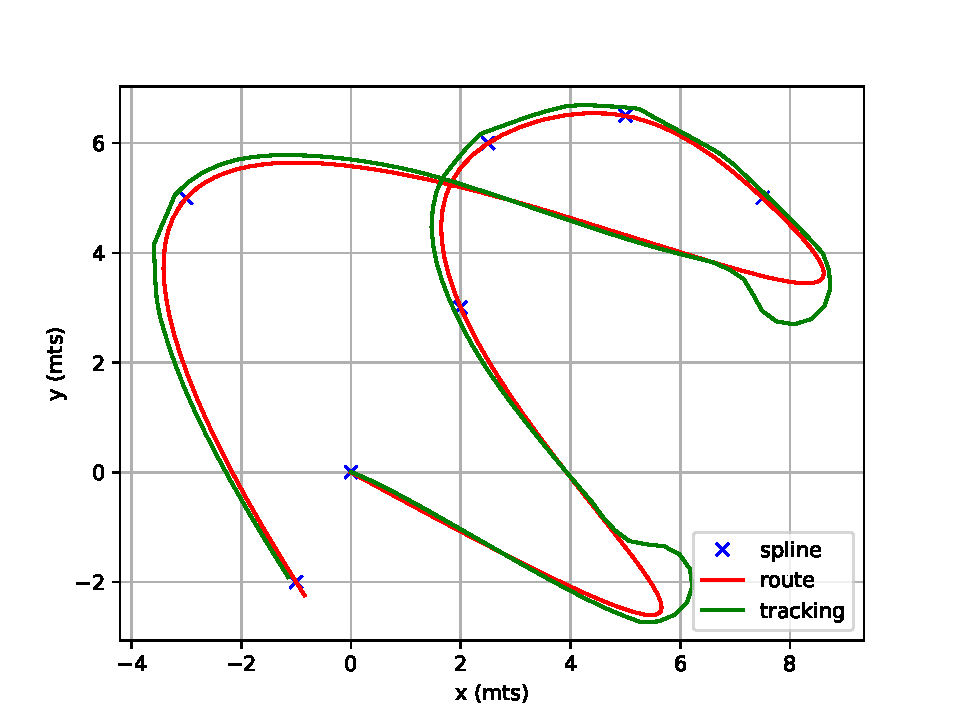
\includegraphics[width=60mm]{img/3r3fmS.pdf}}
    \subfigure[5FM]{\label{fig:compS5FM}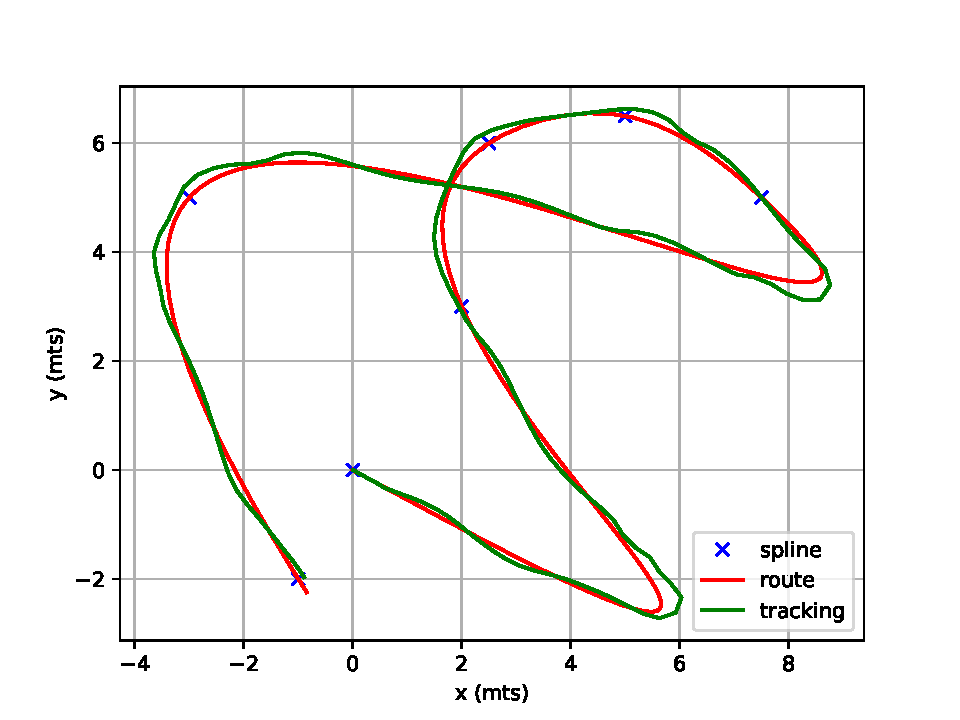
\includegraphics[width=60mm]{img/3r5fmS.pdf}}
     \caption{Plot for the best simulations on Track S}
        \label{fig:3RutasS}
\end{figure}
\begin{paracol}{2}
\linenumbers
\switchcolumn


Finally, in Figure~\ref{fig:yaw} we can have a better look at the steering
motion of each of the controllers concerning the yaw of the ``M'' path. Here we
can see the advantage of the control law. In this case, the 3MF controller has
a very high oscillation, which is not desirable in this type of controller. The
same is observed in the 5MF controller but lesser; this could be related to how
these controllers evolved, giving only weight to $e$.  This is a crucial aspect
to be considered in future work. We can consider including a damping module or
an evaluation metric that negatively weights this kind of oscillation. We can
even include a fuzzy variable to the controller; in comparison, the control law
also uses the curvature of the path $\mathcal{K}(s)$ as a variable for
determining $\omega$.

\end{paracol}
\begin{figure}[h]
    \widefigure
     \centering
    \subfigure[Yaw along the reference path $s(\gamma)$ in meters.]{\label{fig:yawR}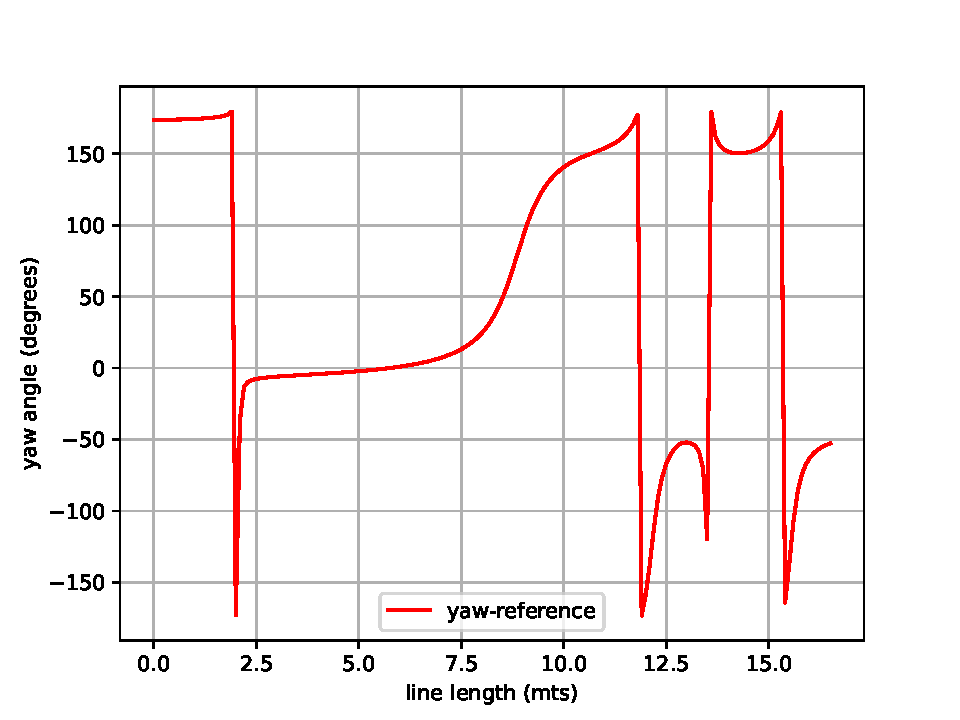
\includegraphics[width=90mm]{img/yawR.pdf}}
    \subfigure[Yaw of the control law as it was tracking the reference path, in seconds.]{\label{fig:yawL}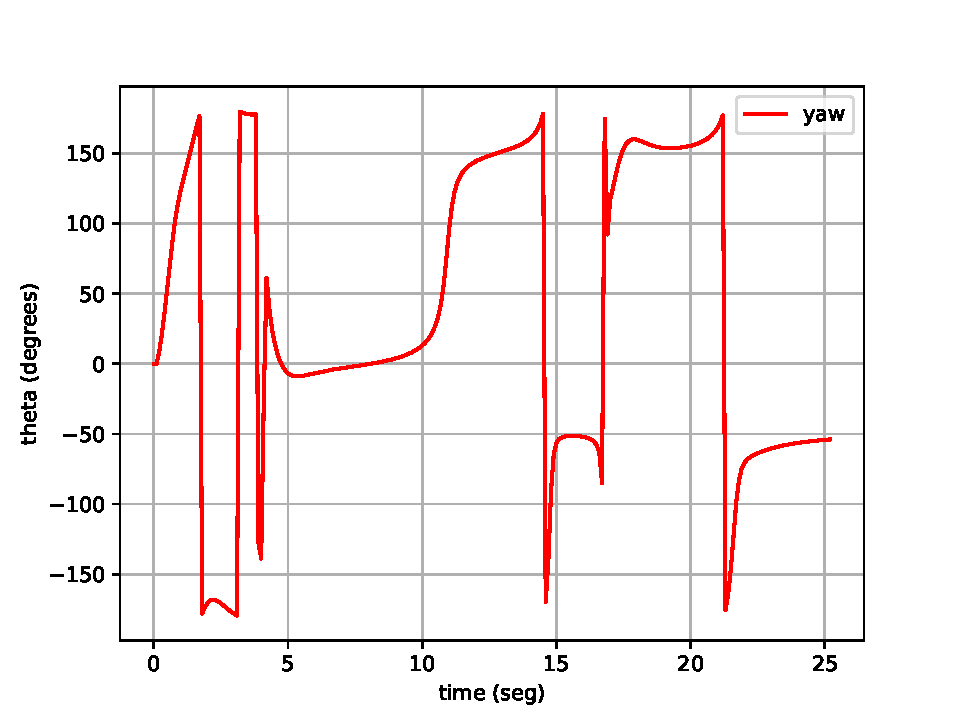
\includegraphics[width=90mm]{img/yawL.pdf}}
    \subfigure[Yaw of the 3MF controller. ]{\label{fig:yaw3}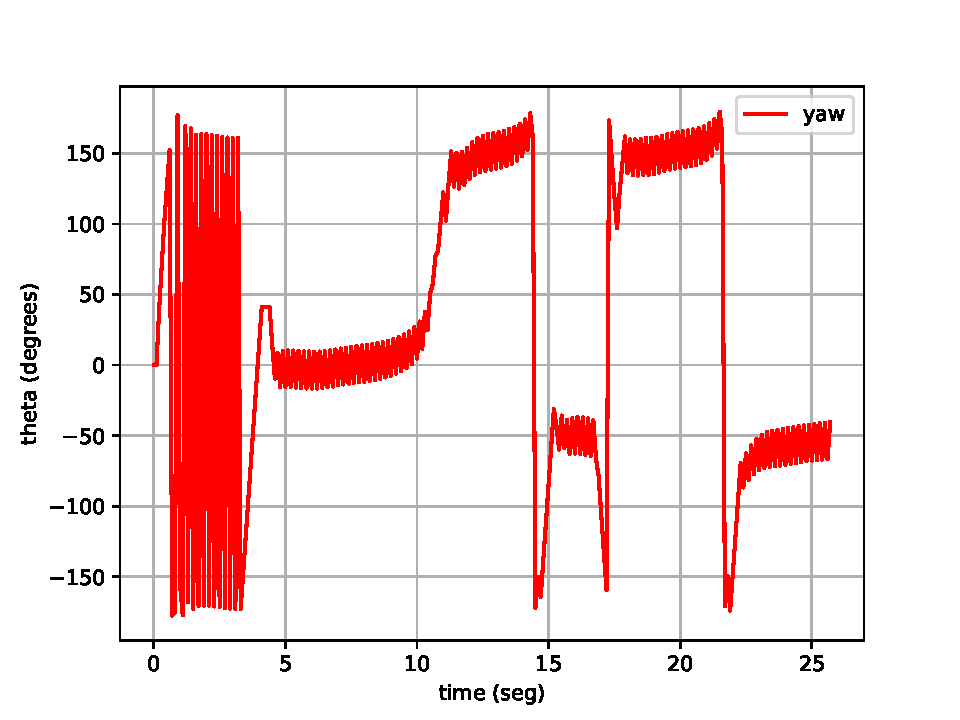
\includegraphics[width=90mm]{img/yaw3.pdf}}
    \subfigure[Yaw of the 5MF controller.]{\label{fig:yaw5}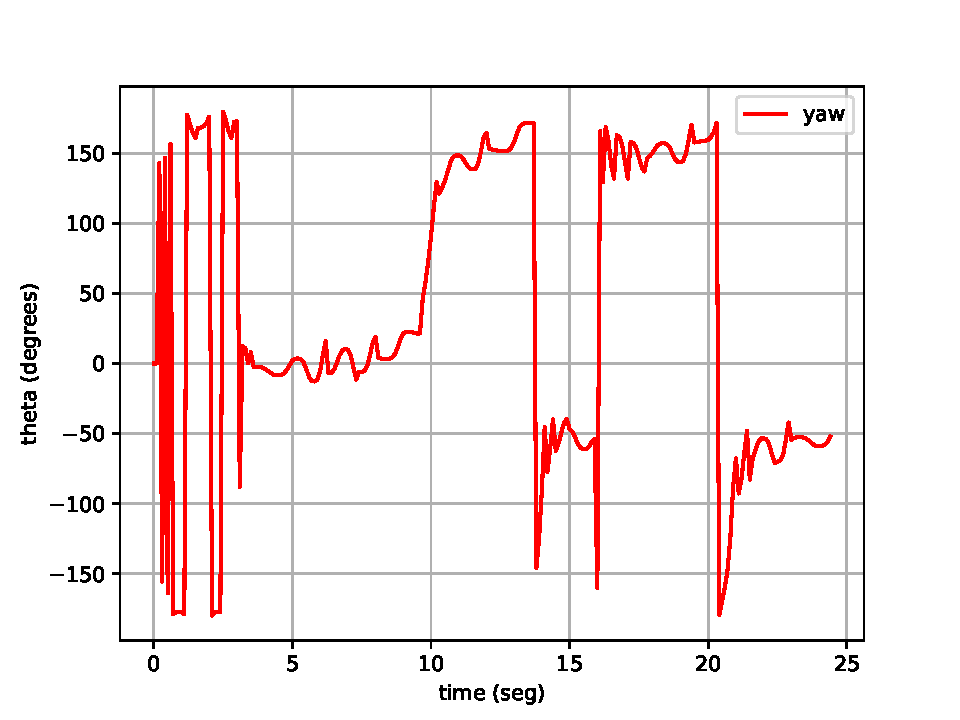
\includegraphics[width=90mm]{img/yaw5.pdf}}
     \caption{Comparison of the yaw (steering) for each of the controllers as it was tracking the reference path ``M'', in seconds.}
        \label{fig:yaw}
\end{figure}
\begin{paracol}{2}
\linenumbers
\switchcolumn
%%%%%%%%%%%%%%%%%%%%%%%%%%%%%%%%%%%%%%%%%%
\section{Discussion}\label{Discussion}

The optimization of fuzzy controllers for real-world applications requires a
broader perspective. We need to treat the problem as a supervised learning
task. The quality of solutions needs to consider other metrics part of the
desired control properties. In this work, experiments show that the overall
result improved by adding a robust validation of candidate solutions. Moreover,
adding more complexity to the knowledge base also improved the control in terms
of RMSE, although needing more computational resources. Our literature review
shows that using only the RMSE is a common practice but could not be enough for
this type of application.

Furthermore, because of the computational cost as future work, we will propose
a technique to execute these experiments in a distributed way. Later we could
try other bio-inspired methods and compare the results. We could also add more
membership functions and test other functions to improve the inference system.

%%%%%%%%%%%%%%%%%%%%%%%%%%%%%%%%%%%%%%%%%%%\section{Conclusions}

%This section is not mandatory, but can be added to the manuscript if the
%discussion is unusually long or complex.

%%%%%%%%%%%%%%%%%%%%%%%%%%%%%%%%%%%%%%%%%%
%\section{Patents}
%
%This section is not mandatory, but may be added if there are patents resulting
%from the work reported in this manuscript.
%
%%%%%%%%%%%%%%%%%%%%%%%%%%%%%%%%%%%%%%%%%%
\vspace{6pt} 

%%%%%%%%%%%%%%%%%%%%%%%%%%%%%%%%%%%%%%%%%%
%% optional
%\supplementary{The following are available online at \linksupplementary{s1}, Figure S1: title, Table S1: title, Video S1: title.}

% Only for the journal Methods and Protocols:
% If you wish to submit a video article, please do so with any other supplementary material.
% \supplementary{The following are available at \linksupplementary{s1}, Figure S1: title, Table S1: title, Video S1: title. A supporting video article is available at doi: link.} 

%%%%%%%%%%%%%%%%%%%%%%%%%%%%%%%%%%%%%%%%%%

\authorcontributions{
Conceptualization, A.M., M.G, and O.C.;
methodology, A.M.; software, M.G.; validation, O.C. and J.M.; data curation, A.M.;
writing---original draft preparation, A.M.; writing---review and editing, M.G. and J.M ;
visualization, A.M.; supervision, O.C.; All authors have read and agreed to the published version of
the manuscript.}

\funding{This research was funded by projects TecNM-5654.19-P and DeepBio (TIN2017-85727-C4-2-P)}

\institutionalreview{Not applicable}

\informedconsent{Not applicable} 

\dataavailability{All data and code is available with an open source license from \url{https://github.com/mariosky/fuzzy-control}} 

%\acknowledgments{In this section you can acknowledge any support given which is not covered by the author contribution or funding sections. This may include administrative and technical support, or donations in kind (e.g., materials used for experiments).}

\conflictsofinterest{``The authors declare no conflict of interest.''} 


%%%%%%%%%%%%%%%%%%%%%%%%%%%%%%%%%%%%%%%%%%
%% Only for journal Encyclopedia
%\entrylink{The Link to this entry published on the encyclopedia platform.}

%%%%%%%%%%%%%%%%%%%%%%%%%%%%%%%%%%%%%%%%%%
%% Optional
%\abbreviations{Abbreviations}{
%The following abbreviations are used in this manuscript:\\
%
%\noindent 
%\begin{tabular}{@{}ll}
%MDPI & Multidisciplinary Digital Publishing Institute\\
%DOAJ & Directory of open access journals\\
%TLA & Three letter acronym\\
%LD & Linear dichroism
%\end{tabular}}
%
%%%%%%%%%%%%%%%%%%%%%%%%%%%%%%%%%%%%%%%%%%
\end{paracol}
%%%%%%%%%%%%%%%%%%%%%%%%%%%%%%%%%%%%%%%%%%
% To add notes in main text, please use \endnote{} and un-comment the codes below.
%\begin{adjustwidth}{-5.0cm}{0cm}
%\printendnotes[custom]
%\end{adjustwidth}
%%%%%%%%%%%%%%%%%%%%%%%%%%%%%%%%%%%%%%%%%%
\reftitle{References}

% Please provide either the correct journal abbreviation (e.g. according to the “List of Title Word Abbreviations” http://www.issn.org/services/online-services/access-to-the-ltwa/) or the full name of the journal.
% Citations and References in Supplementary files are permitted provided that they also appear in the reference list here. 

%=====================================
% References, variant A: external bibliography
%=====================================
\externalbibliography{yes}
\bibliography{tracking}

\end{document}

